\label{sec:dataset}

\subsection{The Human Brain Database Dataset}

The dataset we have worked with for this project comes from the Human Brain Database project. In total it is about 1 TB in size. It consists of a collection of different brain scans from different sources, each of different resolutions and shapes. Due to the size of this dataset we have not yet accessed all of it. 

So far we have only worked with a small subset in order to test our methods. This subset is significantly smaller and is sourced from the SPM Anatomy toolbox \cite{SPMAnatomyToolbox:website}. It has a size of under 10 MB and is a brain atlas consisting of 27 different brain scans. Each scan has a resolution of about $150$ x $150$ x $200$ pixels. 

\subsection{Neuroimaging methods}

Before we describe the dataset in more detail we briefly introduce the reader to the most commonly used neuroimaging methods. This provides the neccessary background to understand what the data means. Neuroimaging is the process of scanning the brain and generating images of it. There are two different methods that are commonly used to achieve this. 

X-ray computed tomography (commonly known as CT scan) is a method which produces multiple two-dimensional X-Ray images of an object to be scanned. With the help of computers these images are then assembled into a full three-dimensional scan. This allows to look inside an object without having to physically disassemble or open it. 

Another common technique is called Magnetic resonance imaging and also known as an MRI scan. MRI scans do not use X-Rays to investigate an object but instead abuse the quantum spin of atoms. By applying a magnetic field, the spins of atoms are forced to align. Once this magnetic field is removed, the atoms return to equilibrium and produce very faint RF emissions. These can be detected, measured and then assembled into a three-dimensional image. 

Both methods produce a 3-dimensional cube with scalar values at each point as the output, although MRI scans usually give higher resolution than X-Rays. For this reason our dataset consists mostly of MRI scans. 

\subsection{The HDF format and BBIC encoding}

When we first received the dataset it was provided in HDF5 format. HDF stands for Hierarchical Data Format and is a data format that was originally developed at National Center for Supercomputing Applications  and is now mainted by the HDF Group \cite{HDF5:website}. It is designed to store and organize large amounts of data and has two different kinds of objects, datasets and groups. Datasets are multi-dimensional arrays of homogeneous type. Groups are containers for datasets and sub groups. This results in a filesystem-like structure for HDF5 files. 

Even though the data is stored inside an HDF file, it was encoded using the BBIC format. This was an internal format used mostly for an image viewer used by our collaborators. Our collaborators stated that ``the bbic format contains a stack of tiled images of different level/resolution. Our image viewer works just like the Google Maps. Every time we zoom in or out, the viewer sends a query to the image service to retrieve certain tiles of images of certain slice at certain resolution'' \cite{BBIC:about}. This makes it very difficult for us to extract the original three-dimensional cube that represents the brain scan. What makes it even more difficult is the fact that there is very little documentation available because the  ``bbic format was developed by a former colleague who has left for long time before I joined'' \cite{BBIC:dev}.

\subsection{The ATLAS viewer}

The BBIC format is used for the so-called ATLAS viewer. This is based on the imaging service mentioned above and is available at \cite{hbp:atlasviewer}. The viewer allows the user to interactively explore a subset of the Human Brain Database. 

The atlas viewer has three main features: 
\begin{inparaenum}[(1)]
\item selection of different brain scans, 
\item looking at different two-dimensional cuts through the original data (Figure~\ref{fig:atlas_browser}) and
\item overlaying of brain region masks (Figure~\ref{fig:atlas_masks}). 
\end{inparaenum}

\begin{figure}[h]
\centering
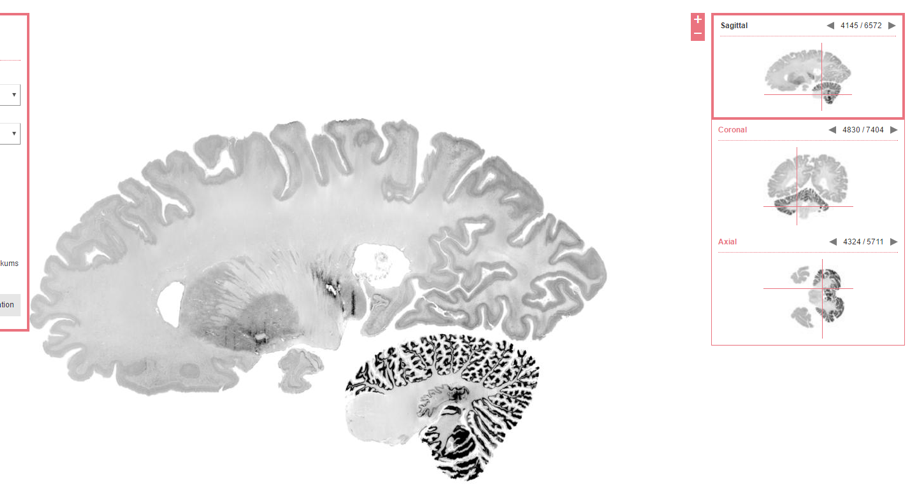
\includegraphics[width=\textwidth]{imgs/atlas_browse}
\caption{A screenshot of the ATLAS viewer showing a basic cut through a single dataset. }
\label{fig:atlas_browser}
\end{figure}

\begin{figure}[h]
\centering
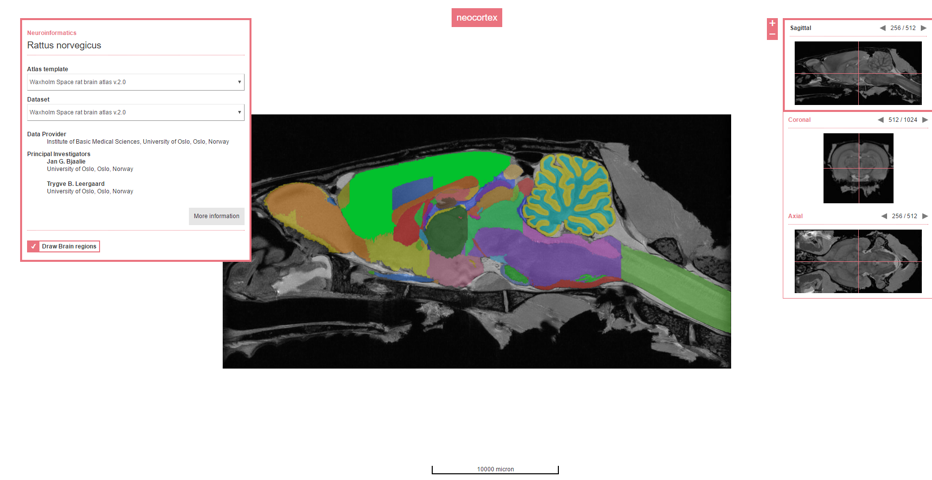
\includegraphics[width=\textwidth]{imgs/atlas_masks}
\caption{A screenshot of the ATLAS viewer showing an overlayed brain region mask. }
\label{fig:atlas_masks}
\end{figure}